% $Header: /Users/joseph/Documents/LaTeX/beamer/solutions/conference-talks/conference-ornate-20min.en.tex,v 90e850259b8b 2007/01/28 20:48:30 tantau $

\documentclass[aspectratio=169]{beamer}
\usepackage{siunitx}
\usepackage[font={footnotesize}]{caption}
\usepackage[
	backend=biber,
	style=authortitle,
	doi=false,
	% isbn=false, 
	maxcitenames=2,
]{biblatex}
\addbibresource{master.bib}

\definecolor{viridis_01}{rgb}{0.267004, 0.048740, 0.329415}
\definecolor{viridis_02}{rgb}{0.190631, 0.407061, 0.556089}
\definecolor{viridis_03}{rgb}{0.208030, 0.718701, 0.472873}
\definecolor{viridis_04}{rgb}{0.993248, 0.906157, 0.143936}

% \AtEveryCite{\color{viridis_03}}

% This file is a solution template for:

% - Talk at a conference/colloquium.
% - Talk length is about 20min.
% - Style is ornate.

% Copyright 2004 by Till Tantau <tantau@users.sourceforge.net>.
%
% In principle, this file can be redistributed and/or modified under
% the terms of the GNU Public License, version 2.
%
% However, this file is supposed to be a template to be modified
% for your own needs. For this reason, if you use this file as a
% template and not specifically distribute it as part of a another
% package/program, I grant the extra permission to freely copy and
% modify this file as you see fit and even to delete this copyright
% notice. 

\mode<presentation>
{
  % \usetheme{default}
  % \usecolortheme{beaver}
  \setbeamercolor{structure}{fg=viridis_01,bg=black!10!}
  % \setbeamercolor{palette secondary}{fg=viridis_02}

  % Remove figure prefix from figures.
  \setbeamertemplate{caption}{\insertcaption} 
}


\usepackage[english]{babel}
% or whatever

\usepackage[latin1]{inputenc}
% or whatever

% \usepackage{times}
\usepackage[T1]{fontenc}
\usepackage{graphics}
\usepackage{caption}
\usepackage{siunitx}
% Or whatever. Note that the encoding and the font should match. If T1
% does not look nice, try deleting the line with the fontenc.

\beamertemplatenavigationsymbolsempty
\usefonttheme{serif}

\title[Short title] % (optional, use only with long paper titles)
{
    Comparison of Simulated Extracellular Spikes from Pyramidal Neurons and Interneurons
}

% \subtitle
% {
% }

\author % (optional, use only with lots of authors)
{Daniel M. Bj\o rnstad}
% - Give the names in the same order as the appear in the paper.
% - Use the \inst{?} command only if the authors have different
%   affiliation.

\date{September 14, 2016}

\institute
{
    Master Thesis Presentation
}




% If you have a file called "university-logo-filename.xxx", where xxx
% is a graphic format that can be processed by latex or pdflatex,
% resp., then you can add a logo as follows:

% \pgfdeclareimage[height=0.5cm]{university-logo}{university-logo-filename}
% \logo{\pgfuseimage{university-logo}}



% Delete this, if you do not want the table of contents to pop up at
% the beginning of each subsection:
%
%\AtBeginSubsection[]
%{
  %\begin{frame}<beamer>{Outline}
  %  \tableofcontents[currentsection,currentsubsection]
  %\end{frame}
%}


% If you wish to uncover everything in a step-wise fashion, uncomment
% the following command: 

%\beamerdefaultoverlayspecification{<+->}


\begin{document}

\begin{frame}
  \titlepage
\end{frame}

%\begin{frame}{Outline}
%  \tableofcontents
  % You might wish to add the option [pausesections]
%\end{frame}


% Structuring a talk is a difficult task and the following structure
% may not be suitable. Here are some rules that apply for this
% solution: 

% - Exactly two or three sections (other than the summary).
% - At *most* three subsections per section.
% - Talk about 30s to 2min per frame. So there should be between about
%   15 and 30 frames, all told.

% - A conference audience is likely to know very little of what you
%   are going to talk about. So *simplify*!
% - In a 20min talk, getting the main ideas across is hard
%   enough. Leave out details, even if it means being less precise than
%   you think necessary.
% - If you omit details that are vital to the proof/implementation,
%   just say so once. Everybody will be happy with that.

% Overview:
%   Motivation and conclusion is very important.
%   This is the first time there have been multiple models of  
%   extracellular potentials have been compared.
%   
%   
% - State the problem?
%       Measuring are often done using tetoredes
% - Goals
%       What can many models of extracellular potentials tell us.
%       Spike width and amp. have been used. Which definition is best.
% - The effects of filtering.
%       Drastically changes spike shape but seperation between neurons can still be seen.
%
% Pictures:
% - Many spikes around a neuron in a grid.
% - Blue brain article

\begin{frame}{Topic and Motivation}
    Topic: Differentiate 2 types of neurons, pyramidal neurons and interneurons, 
    based on extracellular spike shape using computer modelling.
    \newline

    Motivation: 
    \begin{itemize}
        \item Neurons of different types have different functions. Classifying them is important.
        \item Some neurons have shorter spikes than others. 
        \item Electrodes only record electrical potential, they listen in the "dark".
        \item There has been debate wether using spike width can reliably classify neurons. 
    \end{itemize}
\end{frame}

% Firstly I will go through the basic description and function of neurons. 
% Neurons are brain cells bla bla bla. 
\begin{frame}{Theory: What are Neurons}
    \begin{center}
        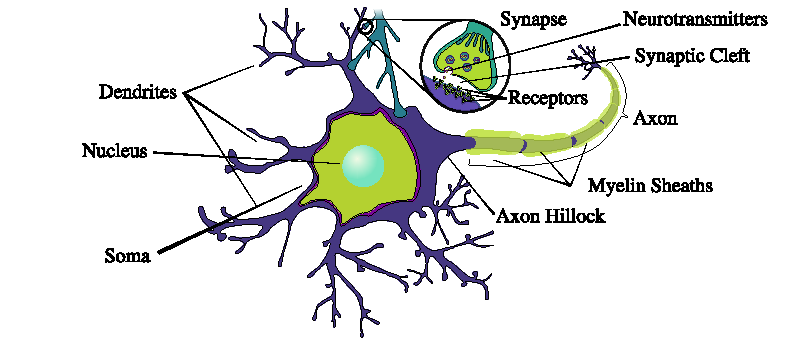
\includegraphics[width=\textwidth]{images/neuron_structure.pdf}
    \end{center}
\end{frame}

% 
% In order to understand how to model these neurons it is necessary
% to know where the electricial activity originates. 
% The neuron membrane consists of bla bla bla. 
% This enables the neuron to create action potentials. 
\begin{frame}{The Neuron Membrane}
    \begin{center}
        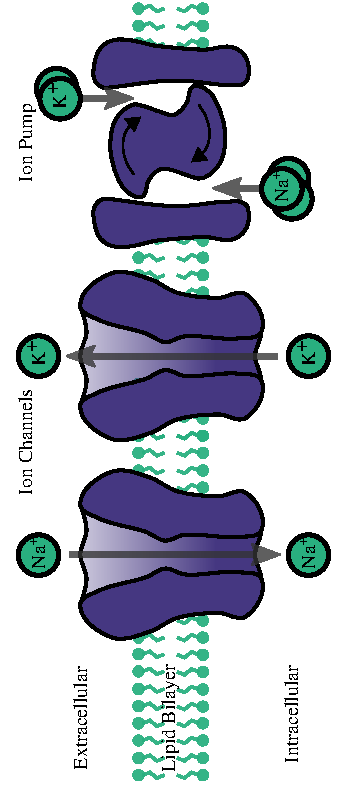
\includegraphics[angle=-90,width=\textwidth]{images/ion_pumps_0.pdf}
    \end{center}
\end{frame}

\begin{frame}{The Membrane Equivalent Circuit: Hudgking and Huxley}
    \begin{center}
        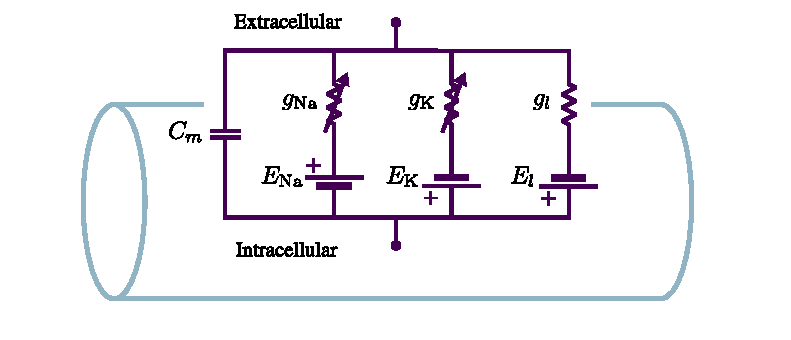
\includegraphics[width=\textwidth]{images/compartment.pdf}
    \end{center}
\end{frame}

\begin{frame}{Action Poential: Toilet Model}
    \begin{columns}
        \begin{column}{0.28\textwidth}
            \begin{center}
                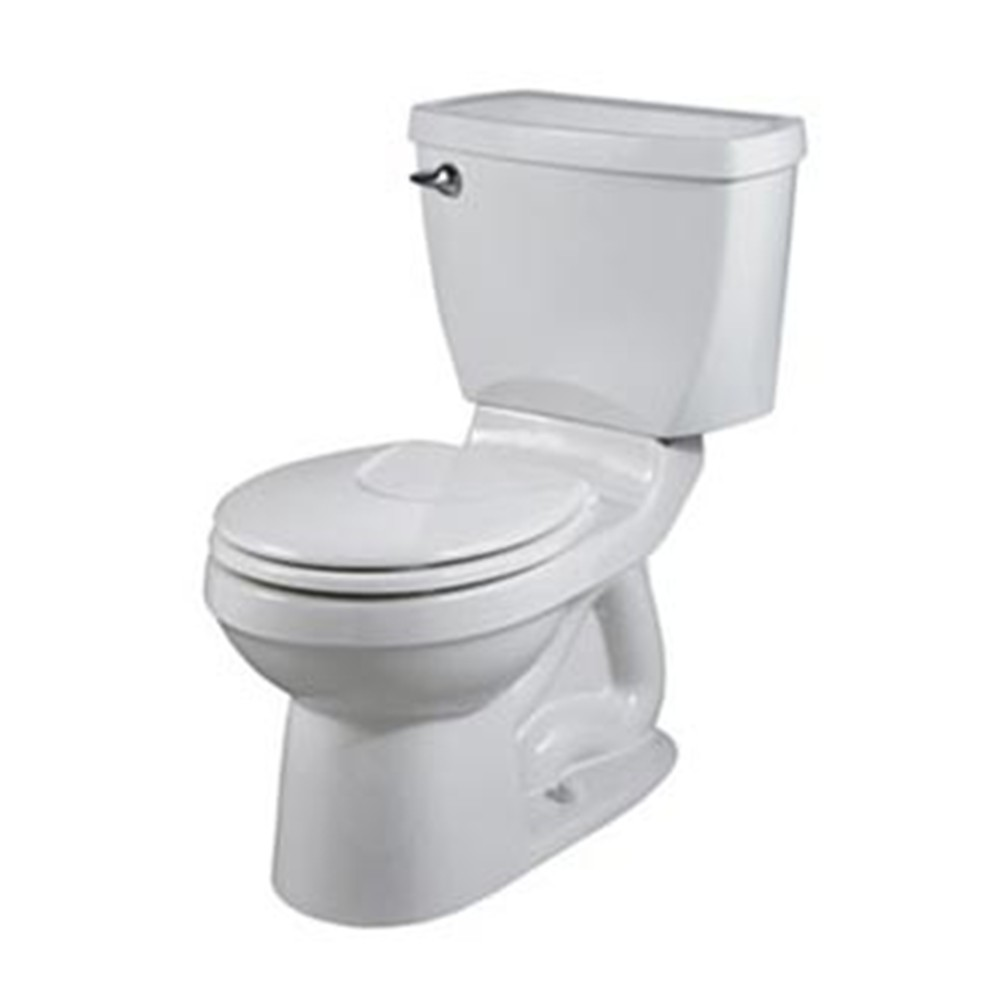
\includegraphics[width=\textwidth]{images/toilet.jpg}
            \end{center}
        \end{column}
        \begin{column}{0.68\textwidth}
            \begin{itemize}
                \item Flushing requires a "strong" push on the button. 
                \item Too little and water will only trickle down. 
                \item When flushed, the intensity is the same every time. 
                \item After a flushing there is a recovery period before we can flush again.
            \end{itemize}
        \end{column}
    \end{columns}
\end{frame}

\begin{frame}{Action Poential: Anatomy}
    \begin{center}
        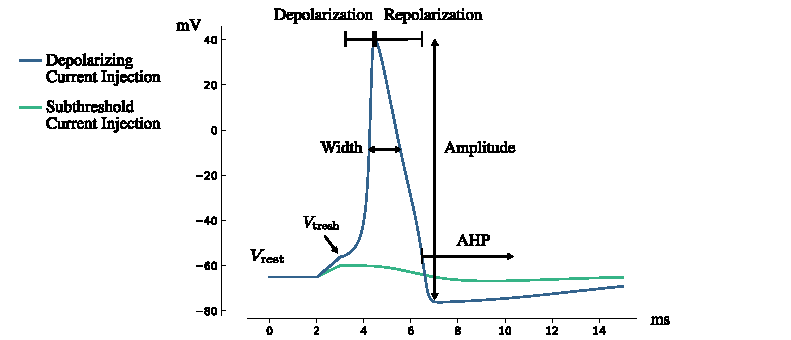
\includegraphics[width=\textwidth]{images/action_potential.pdf}
    \end{center}
\end{frame}

\begin{frame}{Multicompartmental Models}
    \begin{center}
        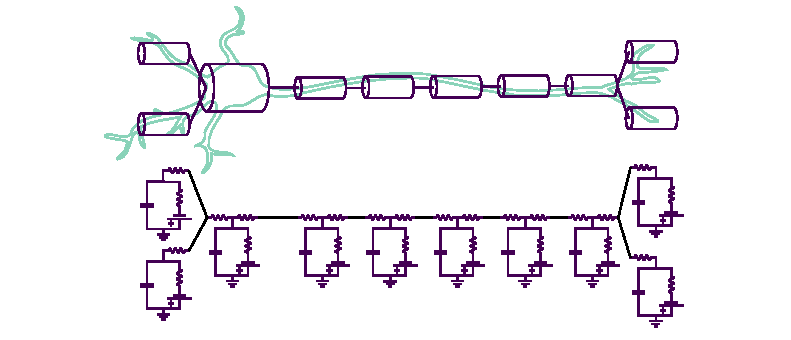
\includegraphics[width=\textwidth]{images/compartments.pdf}
    \end{center}
\end{frame}

\begin{frame}{Extracellular Action Potentials (EAPs)}
    % $$\phi(r, t) = \sum^N_{n=1} \frac{1}{4\pi\sigma}\frac{I_n(t)}{r_n}$$
    % \begin{center}
    %     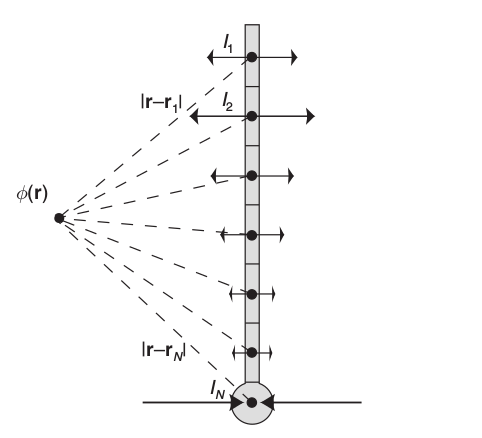
\includegraphics[width=0.5\textwidth]{images/summation.png}
    % \end{center}

    \begin{columns}
        \begin{column}{0.48\textwidth}
            $$\phi(r, t) = \sum^N_{n=1} \frac{1}{4\pi\sigma}\frac{I_n(t)}{r_n}$$
        \end{column}
        \begin{column}{0.48\textwidth}
            \begin{center}
                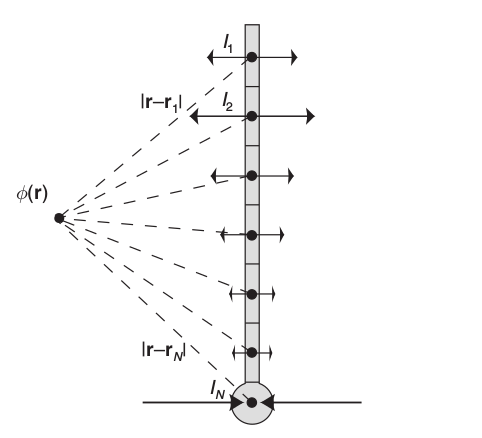
\includegraphics[width=\textwidth]{images/summation.png}
            \end{center}
        \end{column}
    \end{columns}

    % Kirchhoff's current law: All transmembrane currents must sum to 0.
    % When a neurons fires the action potential can be seen outside the cell
    % Also referred to as spikes. 
    % This can be measure by electrodes.
\end{frame}

\begin{frame}{Computer Simulation}
    \begin{center}
        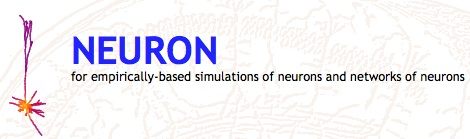
\includegraphics[width=.8\textwidth]{images/neuron_logo.jpg}
        \newline
        
\includegraphics[width=.4\textwidth]{images/LFPy_logo.jpg}
    \end{center}
    % \begin{columns}
    %     \begin{column}{0.48\textwidth}
    %         \begin{itemize}
    %             \item Toilet
    %         \end{itemize}
    %     \end{column}
    %     \begin{column}{0.48\textwidth}
    %         \begin{center}
    %             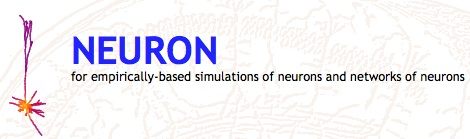
\includegraphics[width=\textwidth]{images/neuron_logo.jpg}
    %             \newline
    %             
\includegraphics[width=.5\textwidth]{images/LFPy_logo.jpg}
    %         \end{center}
    %     \end{column}
    % \end{columns}
\end{frame}

\begin{frame}{EAPs Vary in Shape and Amplitude}
    \begin{center}
        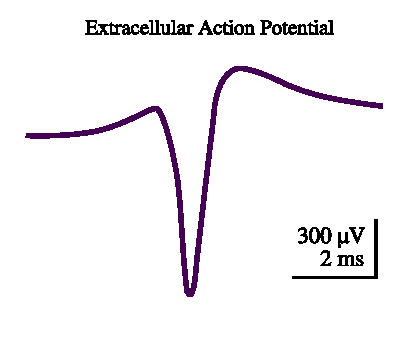
\includegraphics[width=0.5\textwidth]{images/eap.pdf}
        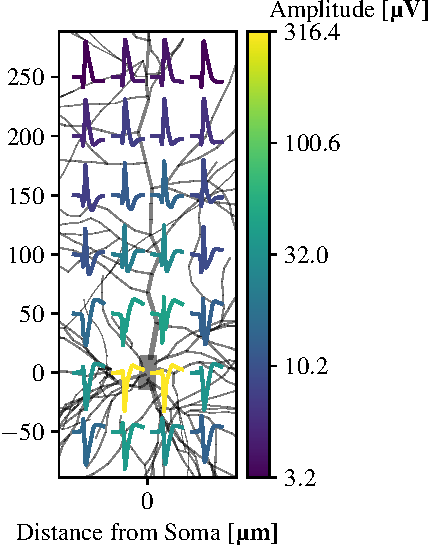
\includegraphics[width=0.4\textwidth]{images/grid_y_x_signals_2d_normalized.pdf}
    \end{center}
\end{frame}

% \begin{frame}{Electrodes}
%     % Single tip electrodes
%     % These are used to measure eap
%     % Introduction to electrodes.
% \end{frame}


\begin{frame}{Spike Width Definition}
    \begin{center}
        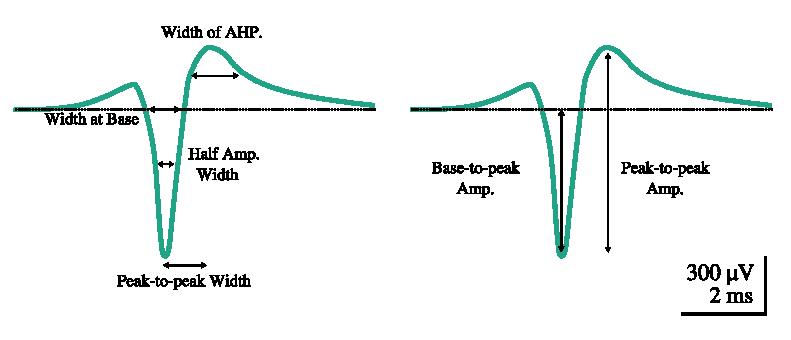
\includegraphics[width=\textwidth]{images/ap_eap.pdf}
    \end{center}
\end{frame}

\begin{frame}{Results Part I: Model Validation}
    Goal: Reproduce spike width and amplitude at increasing distance from soma.
    Setup:
    \begin{itemize}
        \item "Play back" an action potential into soma. 
    \end{itemize}
    \begin{center}
        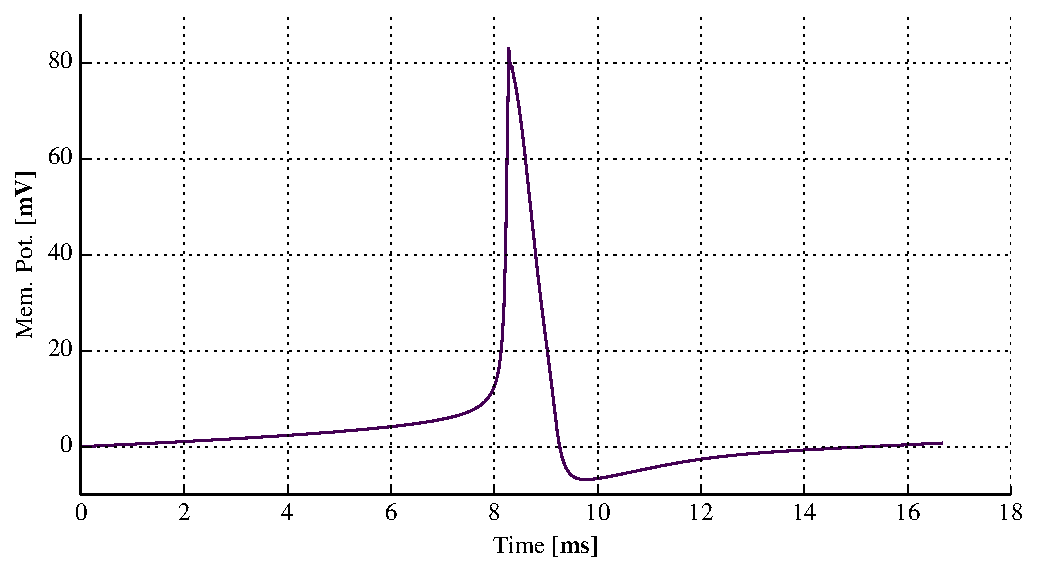
\includegraphics[width=0.5\textwidth]{images/cs_ap_scaled.pdf}
        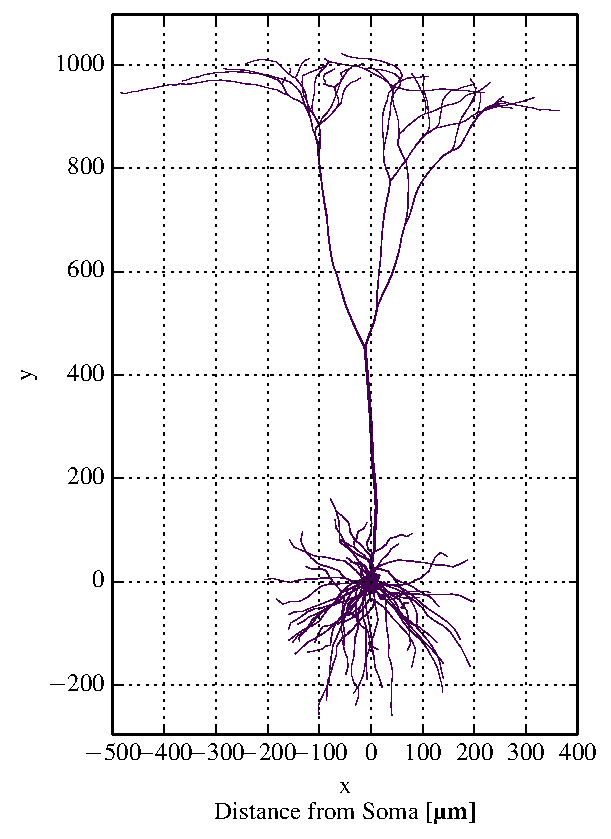
\includegraphics[width=0.2\textwidth]{images/morph_xy_up.pdf}
    \end{center}
\end{frame}

\begin{frame}{Pettersen and Einevoll 2008}
    \begin{columns}
        \begin{column}{0.48\textwidth}
            \begin{itemize}
                \item Electrodes placed in the same way as the article.
                \item Spike width and amplitude measured at every position.
            \end{itemize}
        \end{column}
        \begin{column}{0.48\textwidth}
            \begin{center}
                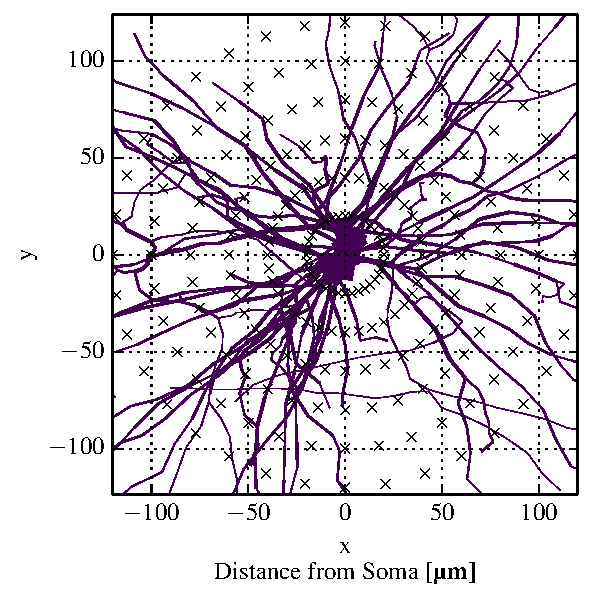
\includegraphics[width=\textwidth]{images/disc_morph_elec_xz.pdf}
            \end{center}
        \end{column}
    \end{columns}
\end{frame}

\begin{frame}{Pettersen and Einevoll 2008}
    \begin{columns}
        \begin{column}{0.48\textwidth}
            \begin{itemize}
                \item Electrodes placed in the same way as the article.
                \item Spike width and amplitude measured at every position.
            \end{itemize}
            Conlusion:
            \begin{itemize}
                \item Results are quantitatively similar. 
            \end{itemize}
        \end{column}
        \begin{column}{0.48\textwidth}
            \begin{center}
                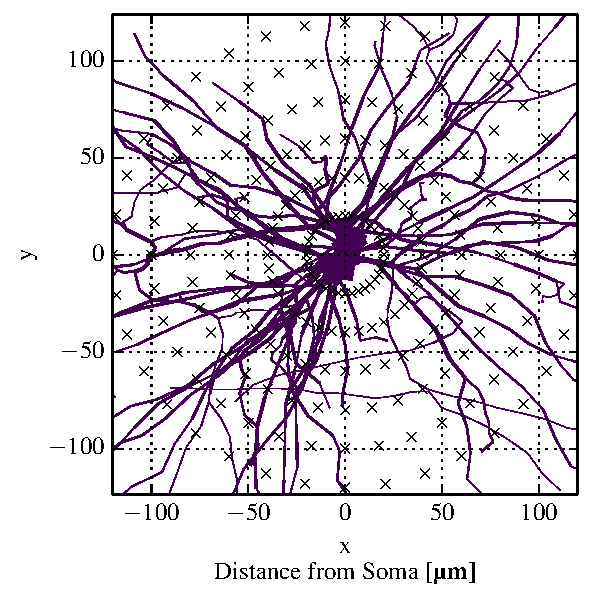
\includegraphics[width=\textwidth]{images/disc_morph_elec_xz.pdf}
            \end{center}
        \end{column}
    \end{columns}
\end{frame}

\begin{frame}{Pettersen and Einevoll 2008}
    \begin{center}
        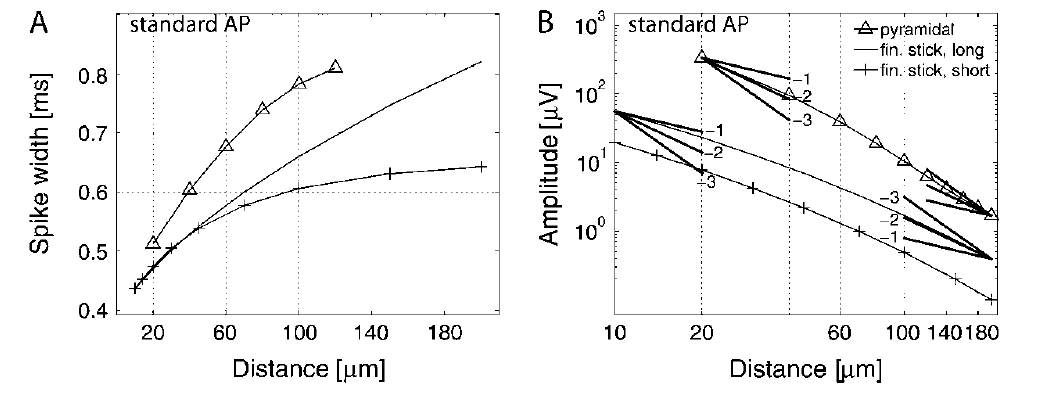
\includegraphics[width=.6\textwidth]{images/pettersen_einevoll.png}
    \end{center}
    \begin{columns}
        \begin{column}{0.48\textwidth}
                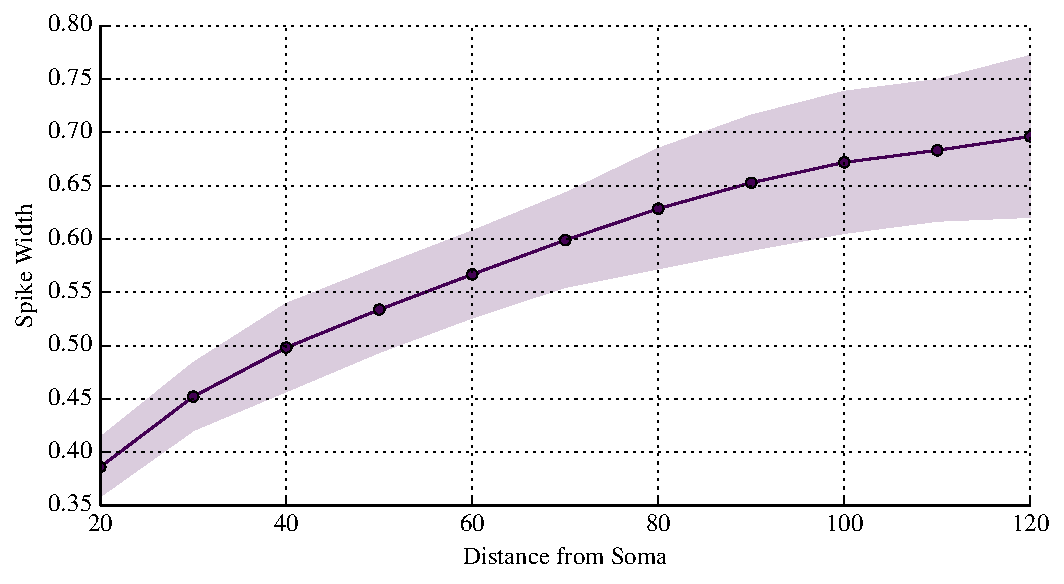
\includegraphics[width=\textwidth]{images/disc_spike_width_II.pdf}
        \end{column}
        \begin{column}{0.48\textwidth}
            \vspace{-1em}
            \begin{center}
                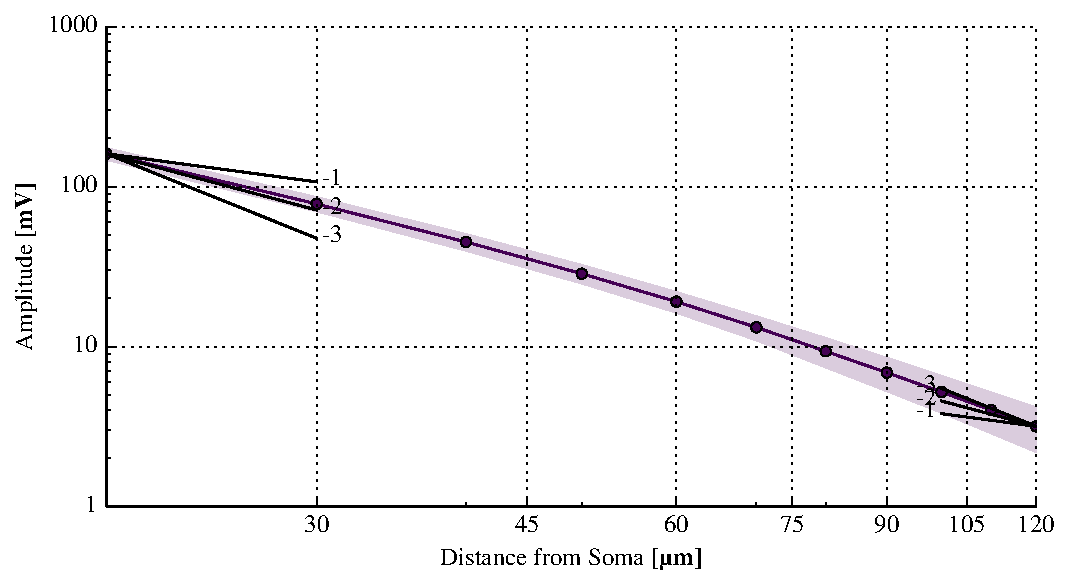
\includegraphics[width=\textwidth]{images/disc_spike_amps_I_log.pdf}
            \end{center}
        \end{column}
    \end{columns}
\end{frame}

\begin{frame}{Results Part II: Comparing Pyramidal Neurons and Interneurons}
    \begin{columns}
        \begin{column}{0.48\textwidth}
            \begin{itemize}
                % \item Many kinds of neurons, their function is not fully known. 
                \item Neurons have commonly been classified by shape (morphology) and
                    electrical activity. 
                \item Pyramidal neuron and interneurons are 2 types based on shape and location.
                \item Though the types have also been associated with other properties
                    such as the spike duration and if they excite other neurons or not.
            \end{itemize}
        \end{column}
        \begin{column}{0.48\textwidth}
            \begin{center}
                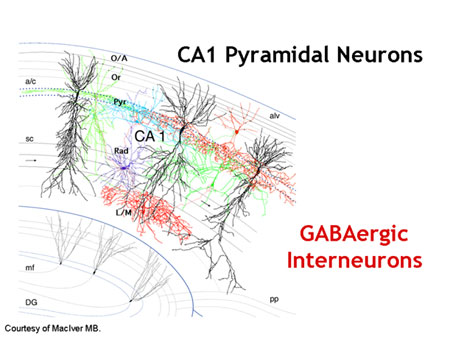
\includegraphics[width=\textwidth]{images/pyr_int_neuron.jpg}
            \end{center}
        \end{column}
    \end{columns}
    % There are many kinds of neurons, but two morphological classes are
    % Pyramidal neurons and interneurons.
    % There has been indications that spikes from interneurons and pyramidal neurons look different.
\end{frame}

\begin{frame}{Goal}
    \begin{itemize}
        \item Does computer models show a difference between interneuron
            and pyramidal neurons.
        \item Are certain width and amplitude definitions better suited for 
            differention.
        \item Can amplitude be used to improve classification.
        \item How does filtering effect the results.
    \end{itemize}
\end{frame}

\begin{frame}{Prior Research}
    \begin{center}
        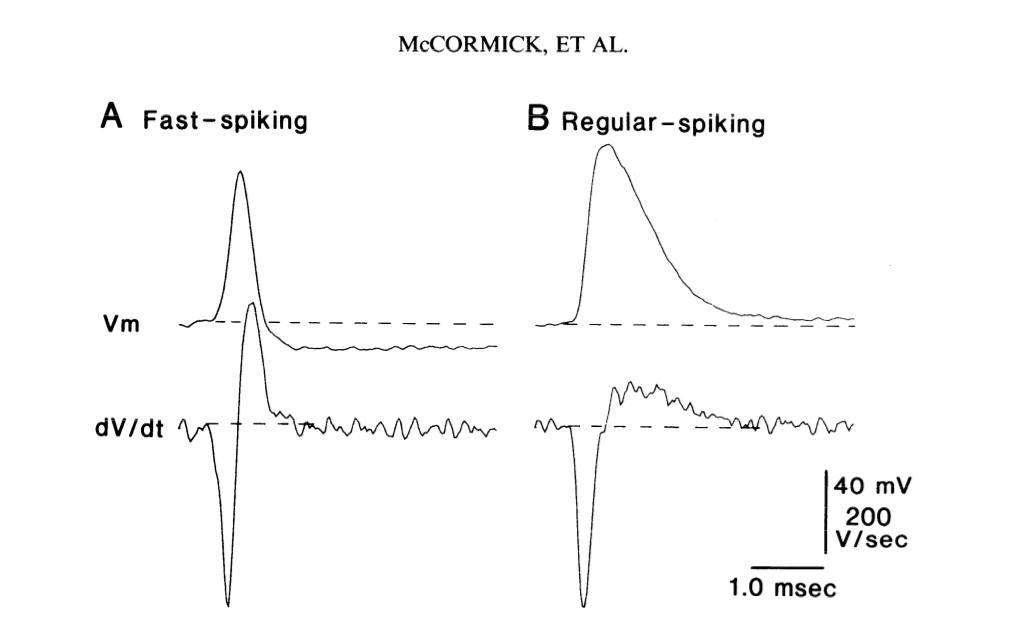
\includegraphics[width=.8\textwidth]{images/mc_cormick_fs_rs.png}
    \end{center}
    % \begin{itemize}
    %     \item Extracellular action potentials (EAP) are unique for each neuron.
    %     \item Was early recoqnized that some interneurons had faster spikes than pyramidal
    %         neurons. 
    % \end{itemize}
\end{frame}

\begin{frame}{Blue Brain Models}
    \begin{center}
        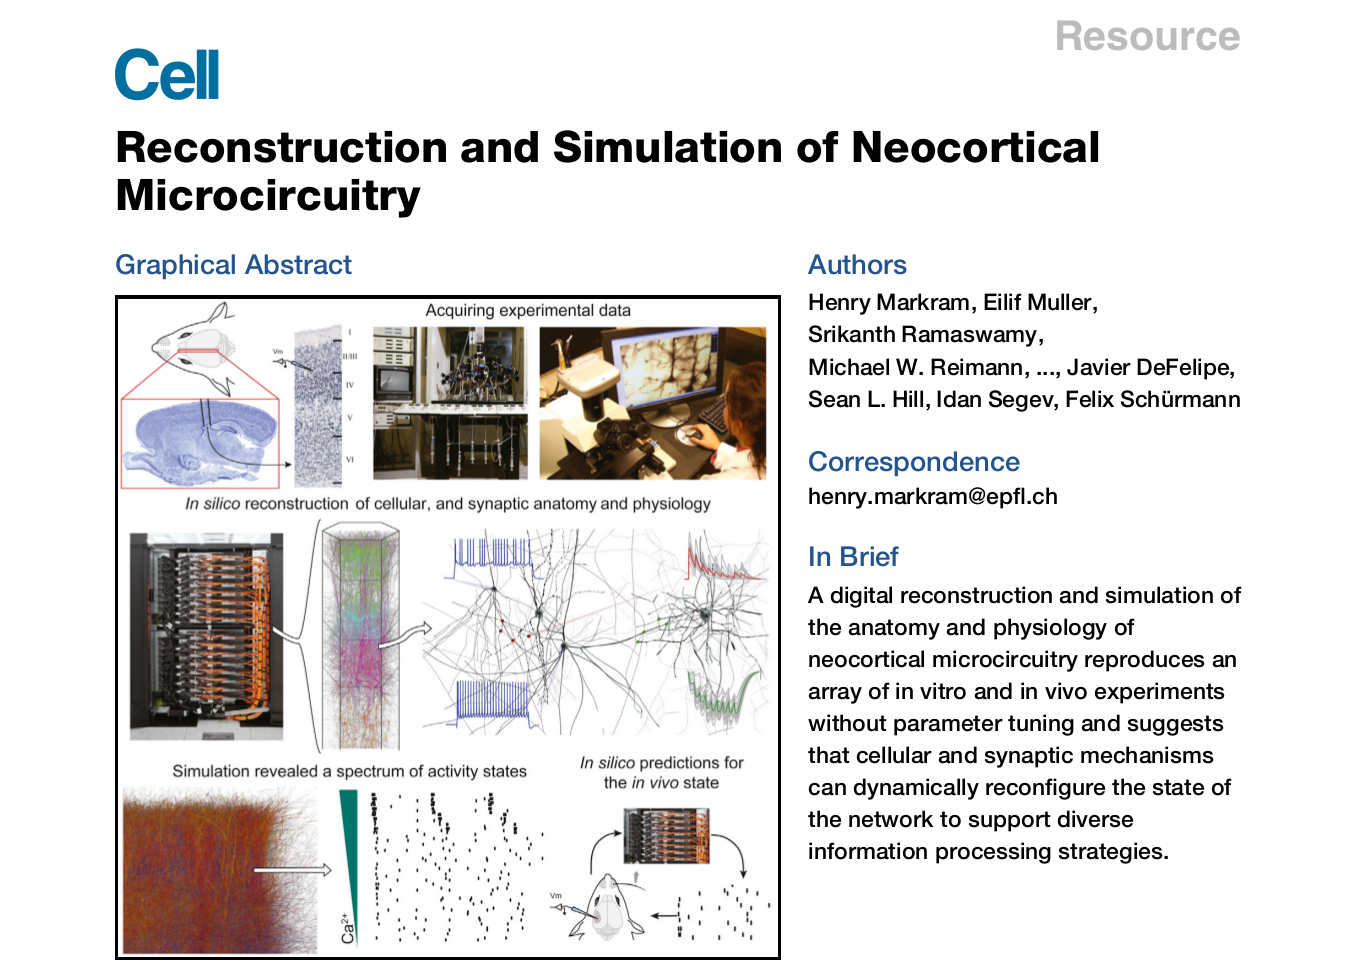
\includegraphics[width=.6\textwidth]{images/markram_front.png}
    \end{center}
\end{frame}

\begin{frame}{Blue Brain M-types}
    \begin{center}
        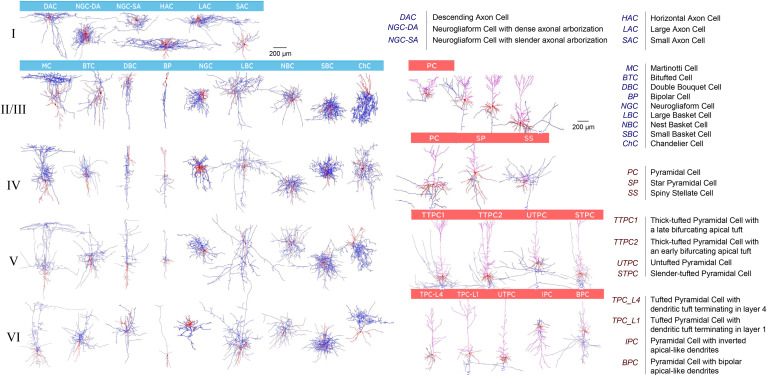
\includegraphics[width=\textwidth]{images/m-types.jpg}
    \end{center}
\end{frame}

\begin{frame}{Blue Brain E-types}
    \begin{center}
        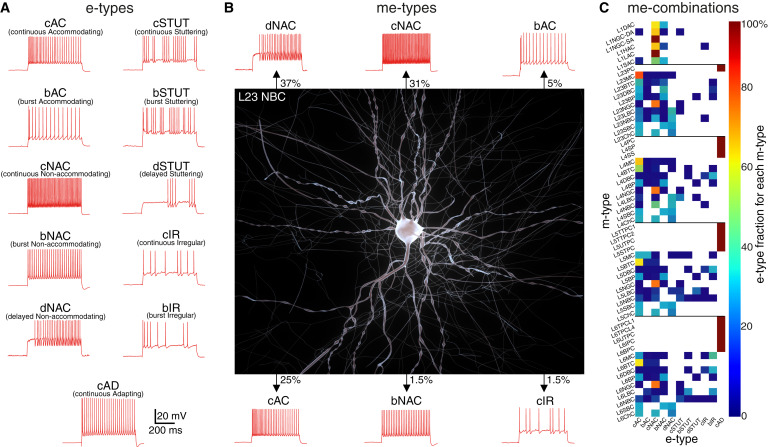
\includegraphics[width=.9\textwidth]{images/e-types.jpg}
    \end{center}
\end{frame}

\begin{frame}{Placing Electrodes}
    % \begin{center}
    %     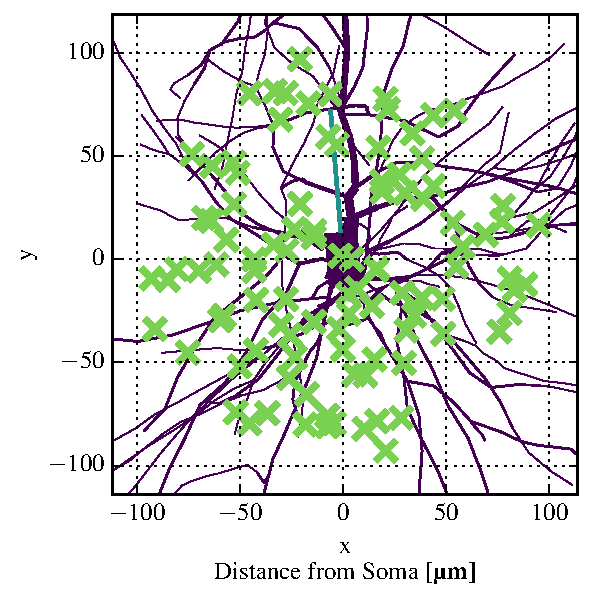
\includegraphics[width=.5\textwidth]{images/sphere_morph_elec_xy.pdf}
    % \end{center}
    \begin{columns}
        \begin{column}{0.28\textwidth}
            \begin{center}
                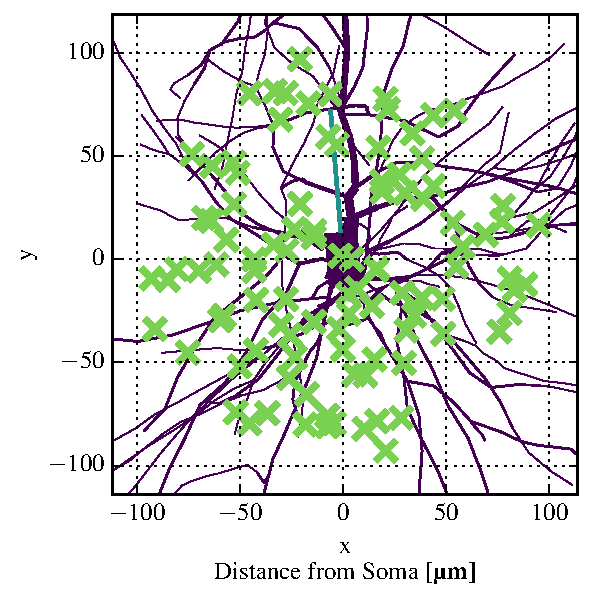
\includegraphics[width=\textwidth]{images/sphere_morph_elec_xy.pdf}
            \end{center}
        \end{column}
        \begin{column}{0.68\textwidth}
            \begin{center}
                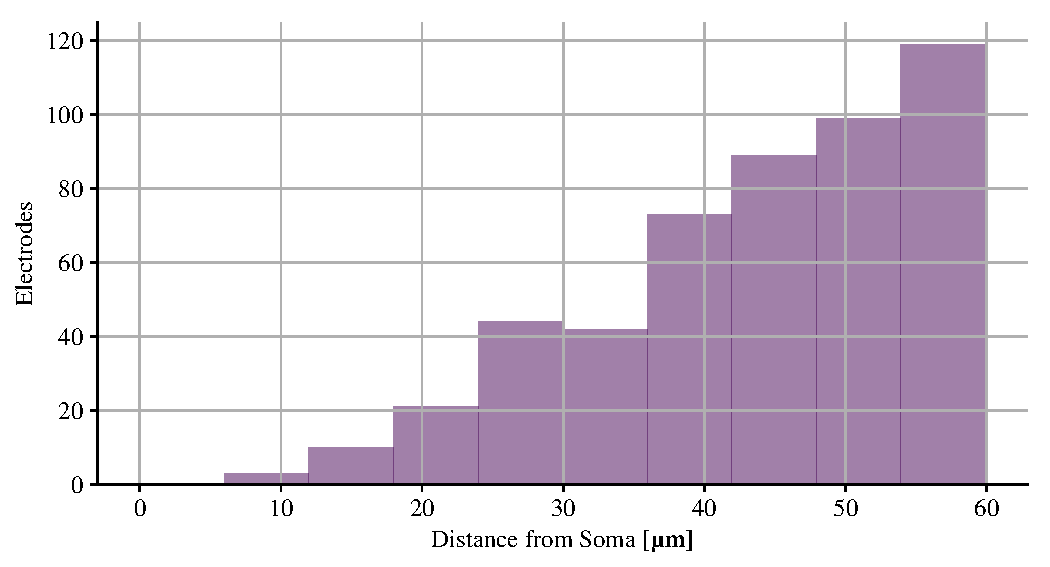
\includegraphics[width=\textwidth]{images/sphere_r_hist.pdf}
            \end{center}
        \end{column}
    \end{columns}
\end{frame}

\begin{frame}{Gather Data}
    % \begin{center}
    %     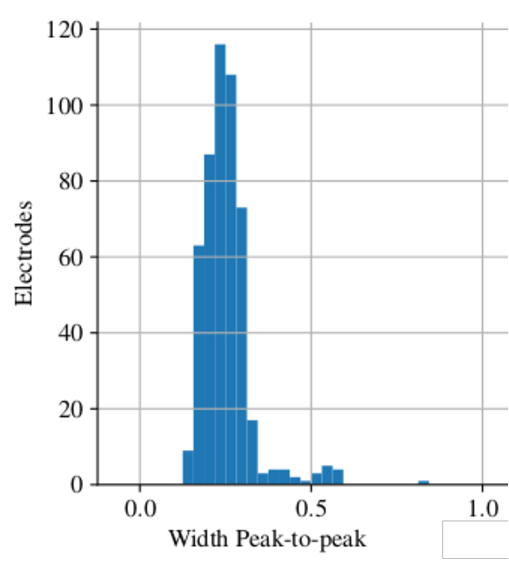
\includegraphics[width=.5\textwidth]{images/sphere_spike_width_II_hist_mod.pdf}
    % \end{center}
    \begin{columns}
        \begin{column}{0.68\textwidth}
            \begin{itemize}
                \item 20 pyramidal models and 240 interneuron models.
                \item Excite the neurons using a square pulse current. 
                \item Record spike width and amplitude using all definitions. 
                \item Binned data into histograms. 
            \end{itemize}
        \end{column}
        \begin{column}{0.28\textwidth}
            \begin{center}
                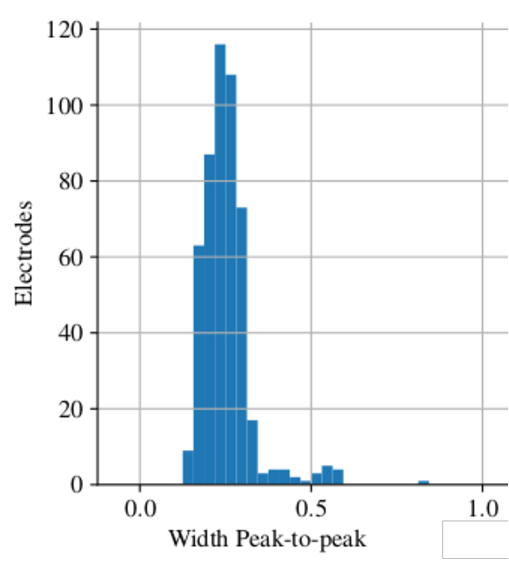
\includegraphics[width=\textwidth]{images/sphere_spike_width_II_hist_mod.pdf}
            \end{center}
        \end{column}
    \end{columns}
\end{frame}

\begin{frame}{Histogram Comparison: ROC Curve}
    \begin{center}
        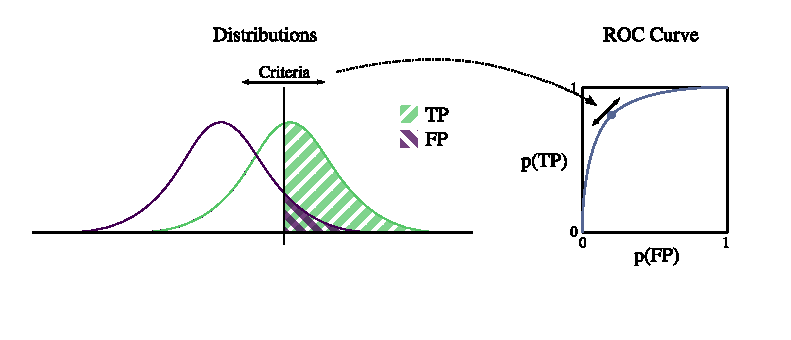
\includegraphics[width=\textwidth]{images/roc_curve.pdf}
    \end{center}
\end{frame}

\begin{frame}{Histogram Comparison: Overlap}
    \begin{center}
        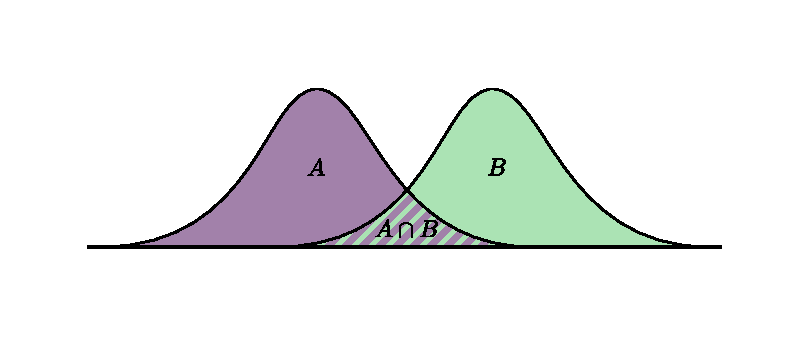
\includegraphics[width=\textwidth]{images/hist_inter.pdf}
    \end{center}
\end{frame}

\begin{frame}{Choosing the Optimal Width Definition}
    \begin{center}
        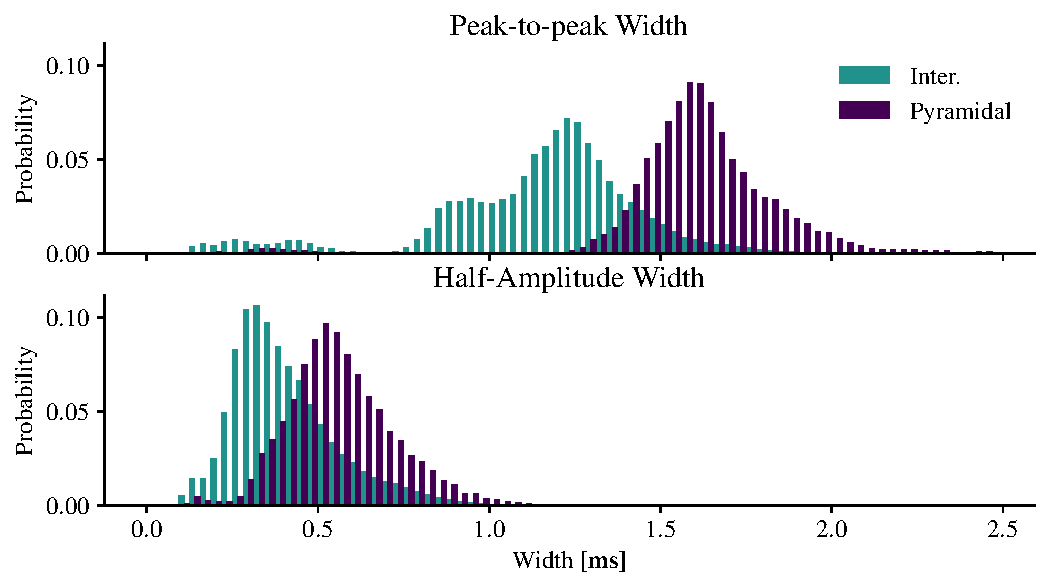
\includegraphics[width=\textwidth]{images/int_pyr_width_I_II.pdf}
    \end{center}
\end{frame}

\begin{frame}{Choosing the Optimal Width Definition}
    \begin{columns}
        \begin{column}{0.48\textwidth}
            \begin{itemize}
                \item ROC area under curve (ROC AUC).
                \item ROC AUC Peak-to-peak: $0.94$.
                \item ROC AUC Half-amp: $0.78$.
            \end{itemize}
        \end{column}
        \begin{column}{0.48\textwidth}
            \begin{center}
                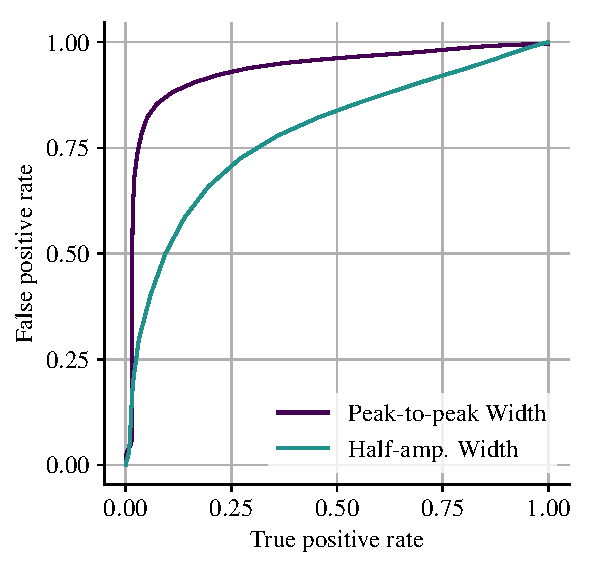
\includegraphics[width=\textwidth]{images/roc_curves.pdf}
            \end{center}
        \end{column}
    \end{columns}
\end{frame}

\begin{frame}{Choosing the Optimal Width Amplitude}
    \begin{center}
        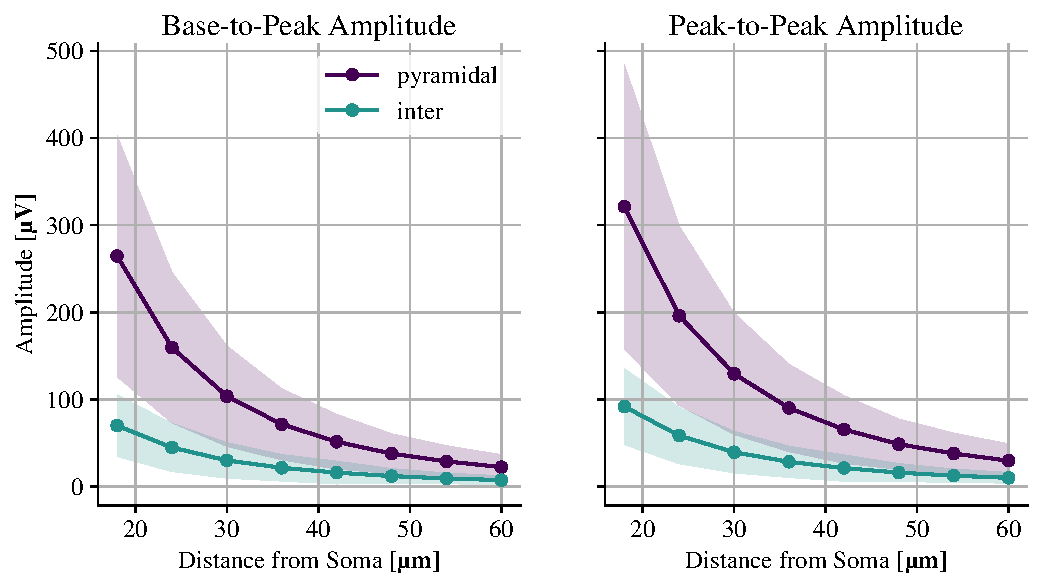
\includegraphics[width=\textwidth]{images/int_pyr_amps_dist.pdf}
    \end{center}
\end{frame}

\begin{frame}{Combining Spike Width and Amplitude}
    \begin{center}
        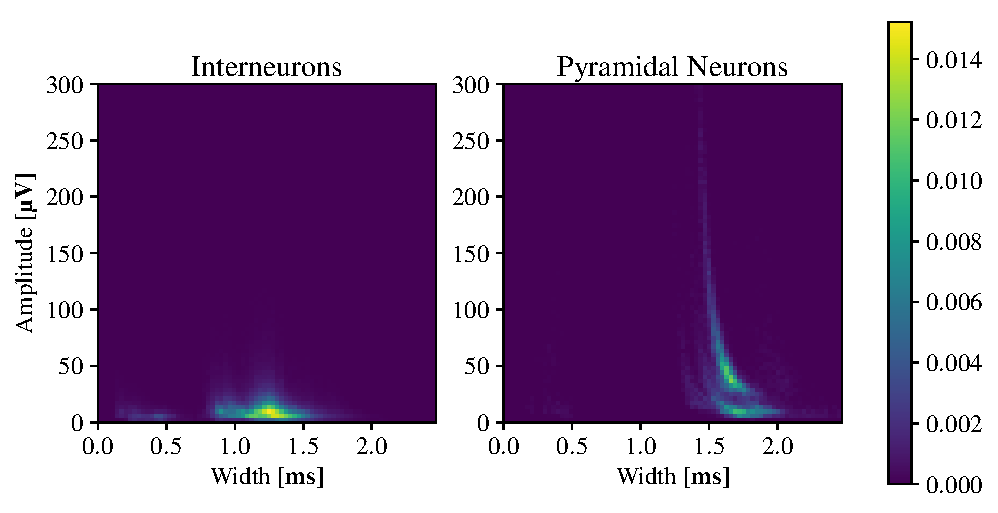
\includegraphics[width=\textwidth]{images/int_pyr_hist.pdf}
    \end{center}
\end{frame}

\begin{frame}{Effects of Filtering}
    \begin{center}
        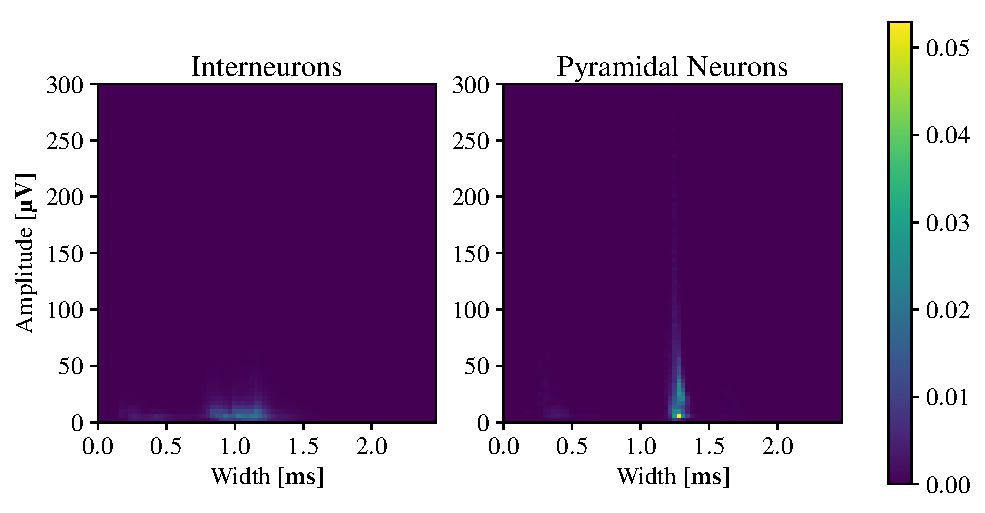
\includegraphics[width=\textwidth]{images/int_pyr_hist_filt.pdf}
    \end{center}
\end{frame}

\begin{frame}[fragile]{Comparison to Other Sources}
    \verb+www.neuroelectro.org+:
    \begin{itemize}
        \item Database of AP data and related properties gather from published articles. 
        \item Intracellular AP half-amp width 
            \SI[separate-uncertainty = true]{1.20 \pm 0.53}{\milli\second}.
        \item Current results found an AP half-amp width of
            \SI[separate-uncertainty = true]{0.70 \pm 0.10}{\milli\second}.
    \end{itemize}
    Anastassiou et al 2015:
    \begin{itemize}
        \item Measured extracellulary and intracellulary at the same time. 
        \item Measured the shape of the AP at increasing firing frequency. 
        \item Current results did not match in shape or value. 
    \end{itemize}
    Bartho et al 2004:
    \begin{itemize}
        \item Measured half-amp and peak-to-peak width. 
        \item Pyramidal neurons: \SI{0.5}{\milli\second} - \SI{1.5}{\milli\second}.
            Current: $>$\SI{1.5}{\milli\second}
        \item Interneurons: \SI{0.2}{\milli\second} - \SI{0.4}{\milli\second}.
            Current: $>$\SI{0.5}{\milli\second}
    \end{itemize}
\end{frame}

\begin{frame}{Summary}
    \begin{itemize}
        \item Reproduced Pettersen and Einevoll 2008. 
        \item Qualitativivly similar but not idenentical. 
        \item Used models from Blue Brain to compare interneurons and pyramidal neurons.
        \item Placed electrodes and gathered data in histograms. 
        \item Spike peak-to-peak width gave better seperation between the types.
        \item Using the spike amplitude gave less overlap, suggesting it is a valuable 
            parameter for classification. 
        \item Seperation still possible after filtering, but values are changed.
    \end{itemize}
\end{frame}

\begin{frame}{Conclusion}
    \begin{itemize}
        \item Modelling EAPs is a valuable tool for neuroscience. 
        \item Supports that spike width can differentiate interneurons and pyramidal neurons.
        \item Certain spike width definitions are better suited for classification.
        \item Spike amplitude increases seperation between interneuron and pyramidal neurons.
    \end{itemize}

    Other remarks: 
    \begin{itemize}
        \item Might be possible to designate areas in the amp. width space to certain kinds
            of neurons. 
        \item LFPy\_util
        \begin{itemize}
            \item Can help the workflow of creating and running simulations.
            \item Can be used as a template for creating and sharing simulations. 
        \end{itemize}
    \end{itemize}
\end{frame}

\end{document}
